\documentclass[11pt]{article}

\usepackage[portuguese]{babel}
\usepackage[utf8]{inputenc}
\usepackage{amsmath}
\usepackage{graphicx}
\usepackage{float}
\usepackage{subfig}
\usepackage{fixltx2e}
\usepackage[bottom]{footmisc}
\usepackage{listings}
\usepackage{color} 
\usepackage{xargs}                      % Use more than one optional parameter in a new commands
\usepackage[pdftex,dvipsnames]{xcolor}  % Coloured text etc.
\usepackage[colorinlistoftodos,prependcaption,textsize=tiny]{todonotes}
\newcommandx{\unsure}[2][1=]{\todo[linecolor=red,backgroundcolor=red!25,bordercolor=red,#1]{#2}}
\newcommandx{\change}[2][1=]{\todo[linecolor=blue,backgroundcolor=blue!25,bordercolor=blue,#1]{#2}}
\newcommandx{\info}[2][1=]{\todo[linecolor=OliveGreen,backgroundcolor=OliveGreen!25,bordercolor=OliveGreen,#1]{#2}}
\newcommandx{\improvement}[2][1=]{\todo[linecolor=Plum,backgroundcolor=Plum!25,bordercolor=Plum,#1]{#2}}
\newcommandx{\thiswillnotshow}[2][1=]{\todo[disable,#1]{#2}}
\usepackage[font=footnotesize]{caption}

\setcounter{tocdepth}{3}

\numberwithin{equation}{section}

\linespread{1.3}
\usepackage{indentfirst}
\usepackage[top=2cm, bottom=2cm, right=2.3cm, left=2.3cm]{geometry}
\addto\captionsportuguese{\renewcommand{\contentsname}{Índice}}

\begin{document}
	
\begin{titlepage}
\begin{center}
	
\hfill \break
\hfill \break


\includegraphics[width=0.3\textwidth]{./logo}~\\[1cm] 

\textsc{\LARGE Instituto Superior Técnico}\\[0.25cm]
\textsc{\Large Mestrado Integrado em Engenharia Electrotécnica e de Computadores}\\[1.8cm]
\textsc{\huge Electrónica Rápida}\\[0.25cm]

\vspace{6mm}

{\huge \bfseries Projecto e Simulação de Misturadores para Altas Frequências\\[1cm]}

\begin{tabular}{ l l }
	Guilherme Branco Teixeira & \hspace{2mm} n.º 70214 \\
	Maria Margarida Dias dos Reis & \hspace{2mm} n.º 73099 \\
	Nuno Miguel Rodrigues Machado & \hspace{2mm} n.º 74236
\end{tabular}

\vspace{7mm}

Grupo n.º 2 de quarta-feira das 11h00 - 12h30

\vfill

{\large Lisboa, 27 de Maio de 2015}
	
\end{center}
\end{titlepage}

\pagenumbering{gobble}
\clearpage

\tableofcontents
\pagebreak

\clearpage
\pagenumbering{arabic}

\section{Introdução}

Este laboratório tem como objectivo a familiarização com circuitos misturadores para altas frequências com componentes discretos. O projecto do circuito e a sua simulação são dois passos essenciais neste laboratório, tendo como objectivo final o projecto da máscara para fabrico.

As especificações do misturador a construir podem ser consultadas na Tabela \ref{tab:car}, tal como as características do substrato plástico para alta frequência da Taconic (TLY -3-0310-CH/CH), sobre o qual o transístor irá ser implantado. 

\begin{table}[h]
\centering
\caption{Características do misturador e substrato.}
\vspace{-1.5mm}
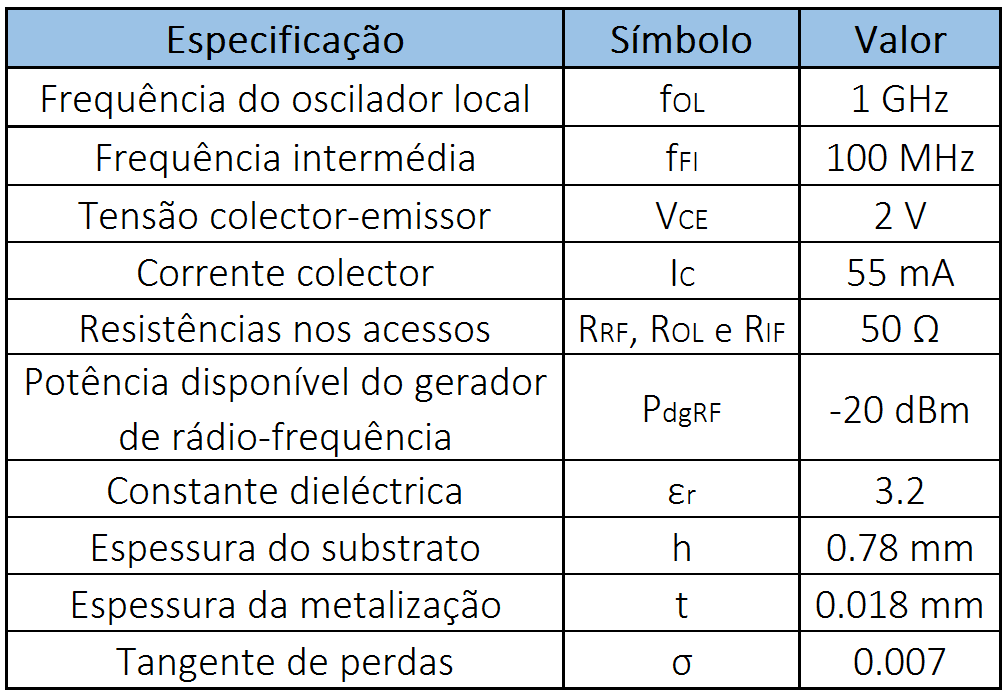
\includegraphics[keepaspectratio=true, scale=0.35]{teoricas/table1}
\label{tab:car}
\end{table}

\section{Misturador com oscilador local na base}

\subsection{Dimensionamento dos componentes}

Numa primeira fase considera-se o circuito da Figura TAL sem filtro de frequência intermédia (FI) e sem malha de adaptação.

\begin{figure}[h]
\centering
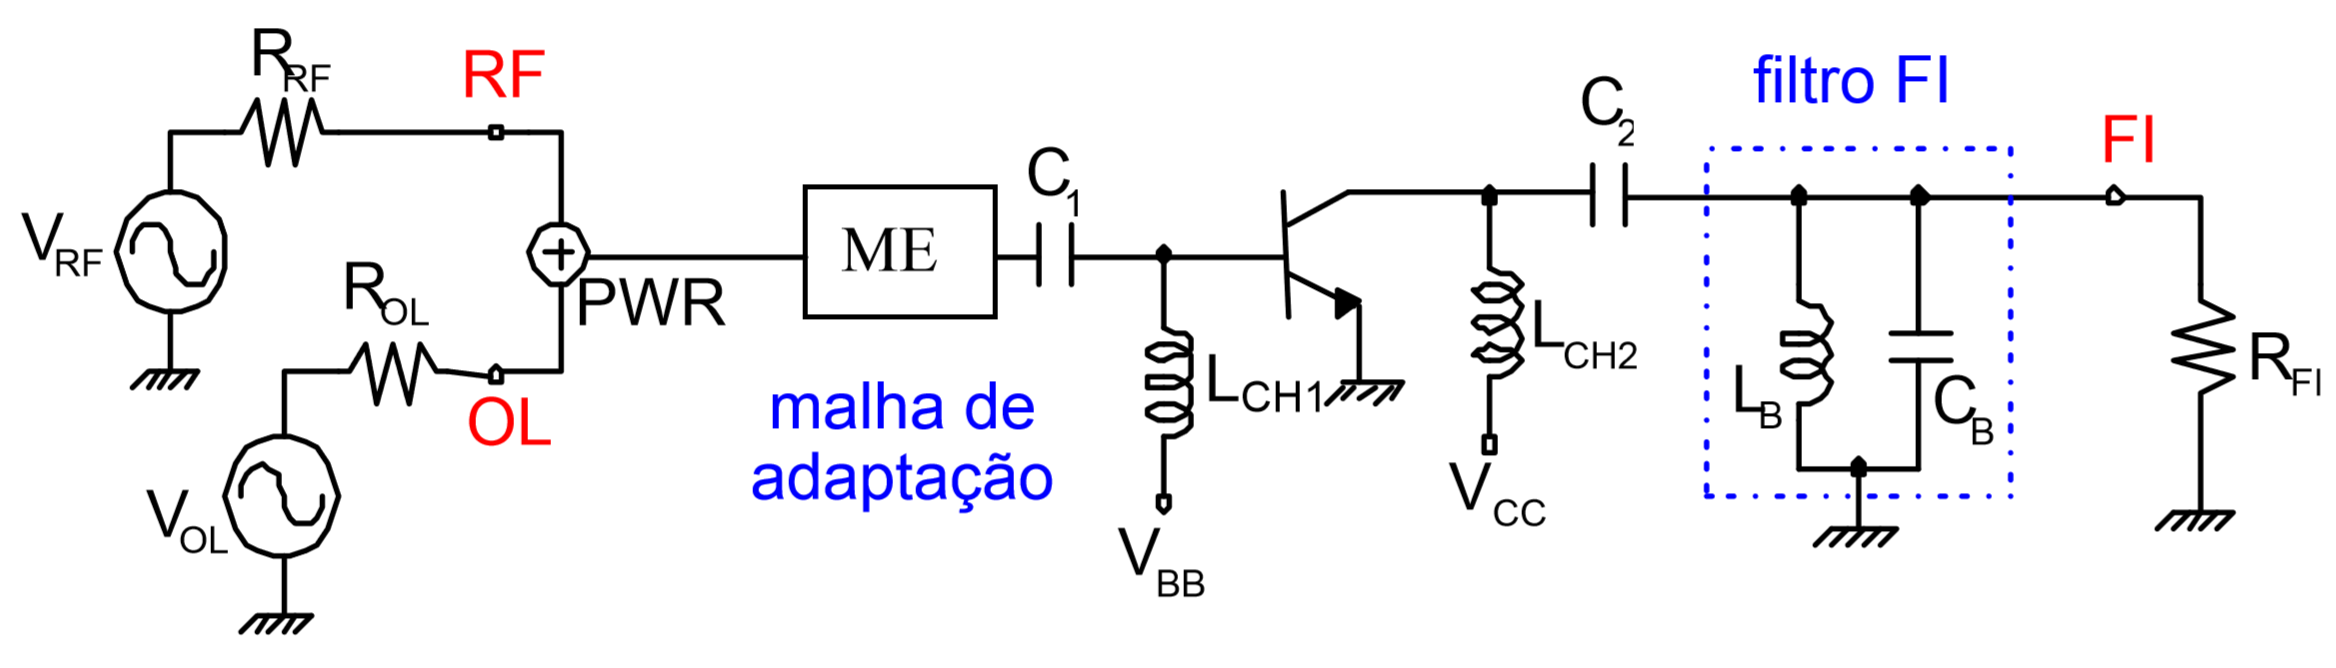
\includegraphics[keepaspectratio=true, scale=0.30]{teoricas/circuitoOriginal}
\vspace{-0.5em}
\caption{Misturador com oscilador local na porta.}
\vspace{-0.8em}
\end{figure}

\paragraph{PFR pretendido} \hspace{0pt} 

Pretende-se determinar os valores das tensões de polarização $V_{BB}$ e $V_{CC}$. Tal como referido na Tabela \ref{tab:car}, as características do ponto de funcionamento em repouso (PFR) já estão pré-definidas, como o valor de $V_{CE}$ e $I_{C}$. Assim, através de uma \texttt{I\_Probe} e fazendo variar os valores de tensão que se pretende calcular, e possível obter os valores que estas tensões assumem quando se obtém o ponto de funcionamento em repouso desejado. Assim,

\vspace{-3mm}
\begin{equation}
\centering
V_{BB} = V_{BE} = 0.72~\text{V} ~ e ~ V_{CC} = 2~\text{V},
\end{equation}

\vspace{1mm} 
valores que foram retirados com recurso à seguinte simulação:

\begin{figure}[h]
\centering
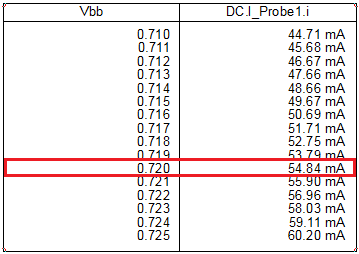
\includegraphics[keepaspectratio=true, scale=0.40]{exps/Vbb}
\vspace{-0.5em}
\caption{Valor do PFR da tensão $V_{BE}$.}
\vspace{-0.8em}
\end{figure}

Para determinar os valores referidos anteriormente, a simulação foi realizada com componentes ideais, nomeadamente as bobines de bloqueio e os condensadores de desacoplamento, no entanto, estes terão de ser dimensionados de modo a que os elementos reais realizem as suas funções sem perturbar o funcionamento do circuito.

Recorrendo às equações \ref{eq:cond_cap} e \ref{eq:cond_ind}, é possível calcular os valores dos condensadores e bobines que respeitem as condições referentes às impedâncias características das linhas de transmissão.

No caso do condensador de desacoplamento DC, $C_{D}$, o seu valor tem de cumprir a condição especificada na equação \ref{eq:cond_cap}, pois sabe-se que a impedância dos condensadores de desacoplamento deve ser bastante inferior à impedância característica das linhas de transmissão. 

\vspace{-3mm}
\begin{equation}
	\lvert Z_C \rvert = \frac{1}{w_{0} C_{D}} << Z_0 \hspace{2mm} \rightarrow \hspace{2mm} C_{D} > \frac{1}{w_{0}Z_0 \times 0.1} \hspace{2mm} \rightarrow \hspace{2mm} C_{D} > \dfrac{1}{5 \times w_{0}}.
	\label{eq:cond_cap}
\end{equation}

\vspace{1mm}
No caso da bobine de bloqueio, $L_{CHK}$, o seu valor tem de cumprir a condição especificada na equação \ref{eq:cond_ind}, pois sabe-se que a impedância das bobines de bloqueio deve ser bastante superior à impedância característica das linhas de transmissão.  

\vspace{-3mm}
\begin{equation}
	\lvert Z_L \rvert = w_{0} L_{CHK} >> Z_0 \hspace{2mm} \rightarrow \hspace{2mm} L_{CHK} > \frac{Z_0 \times 10}{w_{0}} \hspace{2mm} \rightarrow \hspace{2mm} L_{CHK} > \frac{500}{w_{0}}.
	\label{eq:cond_ind}
\end{equation}

\vspace{1mm}

Assim, os valores obtidos para os componentes a dimensionar são:

\vspace{-3mm}
\begin{equation}
\centering
C_{1} > \frac{1}{5 \times 2 \pi \times 1 \times 10^{9}} = 31.83~\text{pF};~ C_{2} > \frac{1}{5 \times 2\pi \times 100 \times 10^{6}} = 318.3~\text{pF}; 
\end{equation}
\vspace{-3mm}
\begin{equation}
\centering
L_{CH1} > \frac{500}{2\pi \times 1 \times 10^{9}} = 79.58~\text{nH};~L_{CH2} > \frac{500}{2\pi \times 100 \times 10^{6}} = 795.8~\text{nH}.
\end{equation}

\vspace{2mm}
As condições dos valores do condensador $ C_{1} $ e da bobine $ L_{CH1} $ foram calculadas com um valor de frequência de 100 MHz, correspondente à frequência $f_{FI}$, pois é esta a frequência esperada nesse ramo do circuito. Já as condições correspondentes ao condensador $ C_{2} $ e à bobine $ L_{CH2} $ foram calculadas com um valor de frequência de 1 GHz, correspondente à frequência $ f_{OL} $, pois é esta a frequência esperada nesse ramo do circuito. Foram escolhidos valores para estes componentes que correspondam a valores de mercado, tal como se pode consultar	 na Tabela \ref{tab:cap_ind}.

\begin{table}[h]
	\centering
	\caption{Valores utilizados para os condensadores de desacoplamento e bobines de bloqueio.}
	\vspace{-1.5mm}
	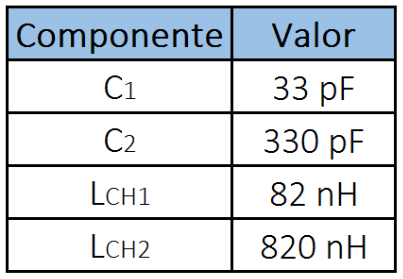
\includegraphics[keepaspectratio=true, scale=0.40]{teoricas/componentes}
	\label{tab:cap_ind}
\end{table}

Relativamente à função destes componentes, a bobine de bloqueio serve para bloquear variações da fonte para o circuito RF, ou seja, desacoplar a componente AC, mas ao mesmo tempo serve para acoplar componente DC. Já o condensador de desacoplamento efectua uma função inversa, ou seja, vai isolar a parte DC mas acoplar a componente AC.

\subsection{Ganho de transdução de conversão}  

O circuito, agora com elementos reais, pode ser simulado. de acordo com o que se pode observar na Figura \ref{fig:Circuito_0}.

\begin{figure}[h]
\centering
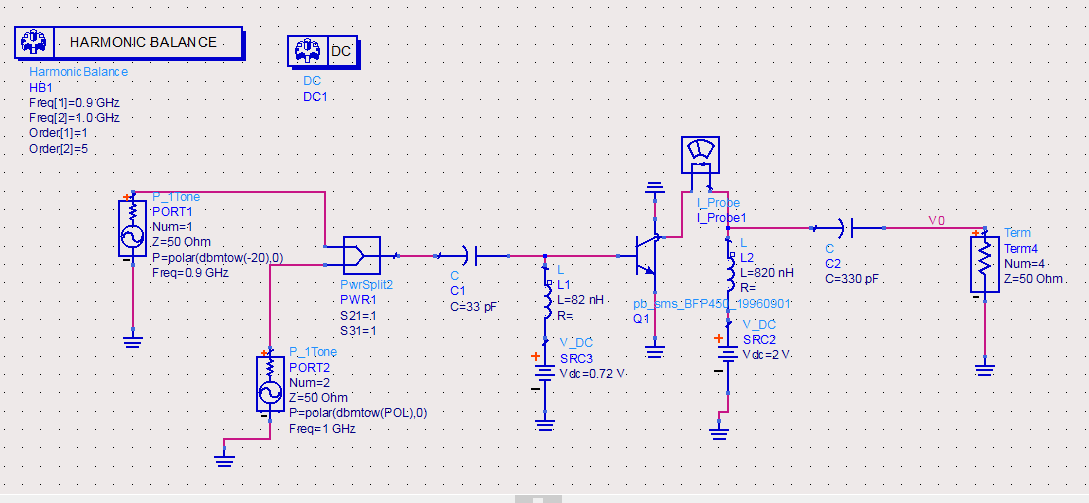
\includegraphics[keepaspectratio=true, scale=0.45]{exps/Circuito_2c}
\vspace{-0.5em}
\caption{Circuito inicial com bobines e condensadores reais.}
\vspace{-0.8em}
\label{fig:Circuito_0}
\end{figure}

O ganho de transdução de um circuito, $G_{TC}$, é a relação entre a potência entregue à carga e a potência disponível no gerador. Havendo conversão, é necessário especificar qual a operação que se está a realizar - neste caso efectua-se uma diferença entre $OL$ e $RF$ para se ter $FI$, ou seja, o valor de $f_{OL}$ é 1 GHz, $f_{FI}$ é 100 MHz e $f_{RF}$ é 900 MHz. 

Simulando o circuito de forma a obter o gráfico do ganho de transdução de conversão deste circuito vem:

\begin{figure}[h]
\centering
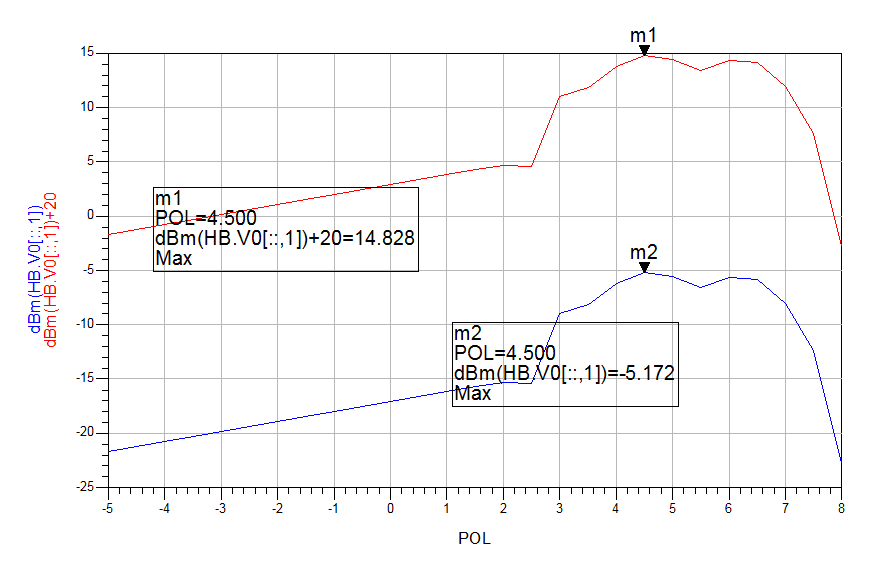
\includegraphics[keepaspectratio=true, scale=0.45]{exps/GT_0}
\vspace{-0.5em}
\caption{Gráfico do ganho de transdução de conversão em função de $ P_{\text{OLDISP}}\left(\omega_{OL}\right) $}.
\vspace{-0.8em}
\label{fig:GT_0}
\end{figure}

Ao observar a Figura \ref{fig:GT_0} é possível determinar o valor de $ P_{\text{OLDISP}}\left(\omega_{OL}\right) $ para qual o ganho de transdução de conversão é máximo, ou seja, 4.5 dBm. Este é o valor óptimo da potência disponível do oscilador local.       

\subsection{Espectros de potência} 

Usando o mesmo circuito da Figura \ref{fig:Circuito_0} foi possível obter o gráfico com os espectros de potência, usando como referência o máximo do ganho de transdução, ou seja, esta simulação foi realizada com um valor fico de $ P_{\text{OLDISP}}\left(\omega_{OL}\right) $, '4.5'.

\begin{figure}[h]
\centering
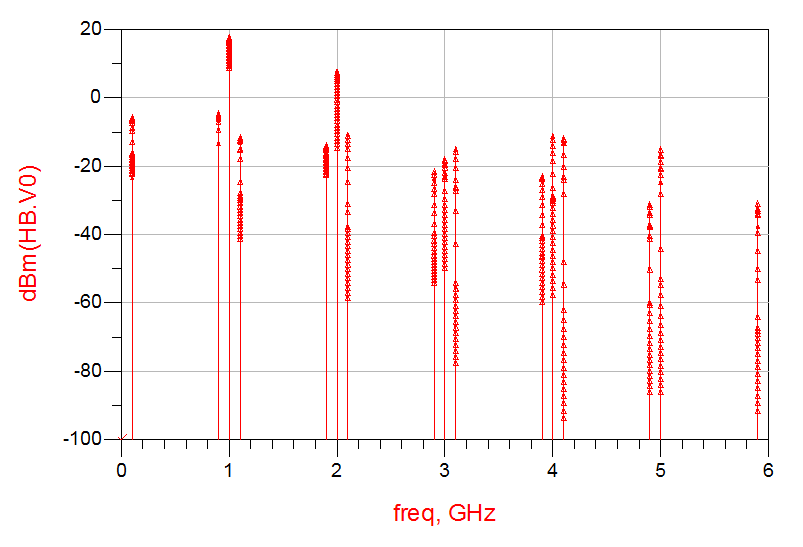
\includegraphics[keepaspectratio=true, scale=0.45]{exps/EP_0}
\vspace{-0.5em}
\caption{Espectros de potência.}
\vspace{-0.8em}
\label{fig:EP_0}
\end{figure}

Na Figura \ref{fig:EP_0}, a risca com o marcador \texttt{m1} corresponde ao espectro de potência da frequência $f_{FI}$, a risca com o marcador \texttt{m2} corresponde ao espectro de potência da frequência $f_{RF}$ e a risca com o marcador \texttt{m3} corresponde ao espectro de potência da frequência $f_{OL}$.

A partir da Figura \ref{fig:EP_0}, pode-se calcular os valores dos isolamentos $OL - RF$ e $OL - FI$. O cálculo corresponde a ir ao porto de FI e ver quanto de OL chega até lá, sendo que idealmente não chegaria nada e o porto seria perfeito. Assim, o que se deve fazer é a diferença entre as componentes espectrais respectivas do isolamento que se está a considerar, ou seja, $I_{\text{OLRF}} = P_{\text{OLDISP}}\left(\omega_{OL}\right) / P_{\text{RF}}\left(\omega_{OL}\right) $ e $I_{\text{OLFI}} = P_{\text{OLDISP}}\left(\omega_{OL}\right) / P_{\text{FI}}\left(\omega_{OL}\right) $.

\begin{table}[h]
	\centering
	\caption{Valor dos isolamentos.}
	\vspace{-1.5mm}
	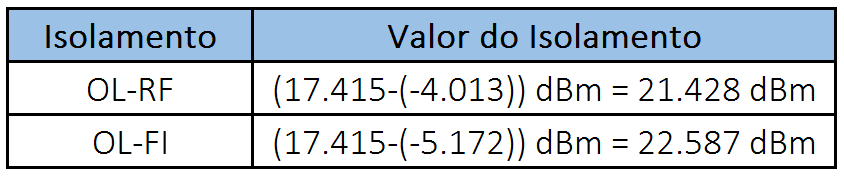
\includegraphics[keepaspectratio=true, scale=0.40]{teoricas/isolamentos}
\end{table}

É também possível a partir dos espectros de potência calcular o valor do ganho de conversão, $G_{PC}$, que corresponde a $ P_{\text{FI}}\left(\omega_{OL}\right)/P_{\text{RF}}\left(\omega_{OL}\right) $. \todo{como calcular?}


\subsection{Filtro de frequência intermédia}

Tem-se como referência o valor da frequência $ f_{FI} $, ou seja, $ \omega_{0}=2\pi f_{FI} $ e um factor de qualidade do filtro de 10. Relativamente ao filtro passa-banda sabe-se que:

\vspace{-3mm}
\begin{equation}
\omega_{0}=\frac{1}{\sqrt{C_{0}L_{0}}} ~ \text{e} ~ B=\frac{1}{R_{FI}C_{0}} ~ \text{e} ~ Q=\frac{\omega_{0}}{B}.
\label{eq:filtro_0}
\end{equation}

\vspace{1mm}
Tendo em conta as expressões na equação \ref{eq:filtro_0}, é possível determinar os componentes que compõem o filtro, Tabela \ref{tab:Comp_filtro}.

\begin{table}[h]
	\centering
	\caption{Componentes que compõem o filtro de FI.}
	\vspace{-1.5mm}
	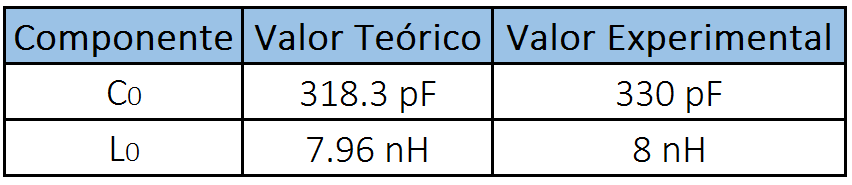
\includegraphics[keepaspectratio=true, scale=0.40]{teoricas/filtro}
	\label{tab:Comp_filtro}
\end{table}

Mais uma vez, os valores resultantes de cálculos teóricos foram substituídos por valores que correspondem a componentes disponíveis no mercado, como se pode ver na tabela anterior quando se refere o valor experimental.

O circuito resultante após a integração do filtro dimensionado pode ser consultado na Figura \ref{fig:Circuito_1}.

\begin{figure}[h]
\centering
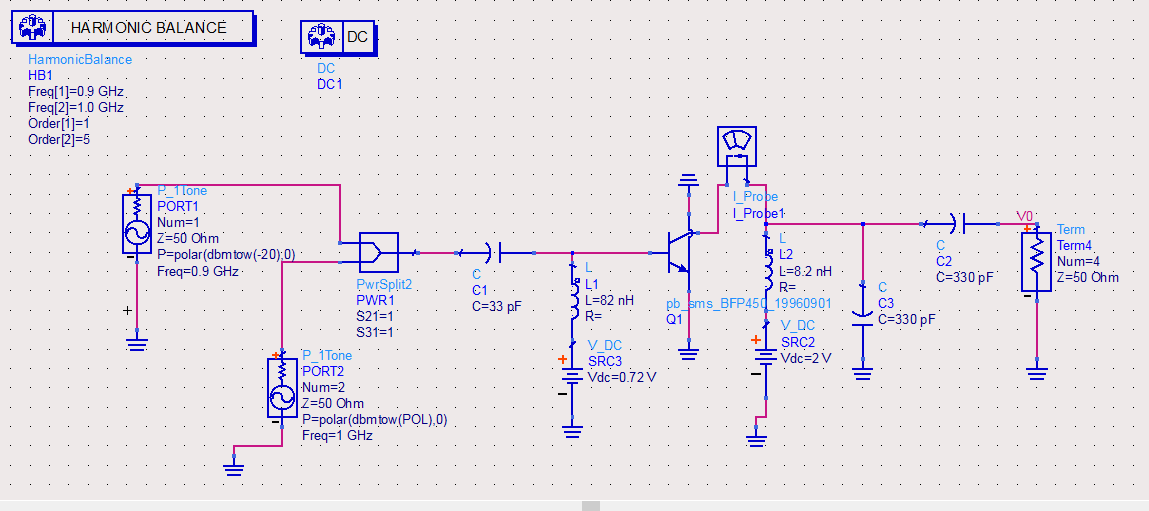
\includegraphics[keepaspectratio=true, scale=0.45]{exps/Circuito_1}
\vspace{-0.5em}
\caption{Circuito após a inserção do filtro de FI.}
\vspace{-0.8em}
\label{fig:Circuito_1}
\end{figure}

Como se pode observar na Figura \ref{fig:Circuito_1}, a bobine de bloqueio $L_{CH2}$ foi substituída pela bobine que compõe o filtro de FI, pois a bobine $ L_{0} $ consegue desempenhar a função da bobine de desacoplamento e, ao mesmo tempo, usa-se uma bobine ao invés de duas, tendo assim diminuído as desvantagens causadas pela presença de bobines num circuito. De facto, poder-se-ia utilizar um filtro passa-baixo, mas o filtro passa-banda tem a vantagem de ter a bobine em paralelo que permite ``reciclar'' a bobine $L_{CH2}$.

É possível agora comparar os gráficos do ganho de transdução de conversão, antes e depois de se acrescentar o filtro ao circuito, Figura \ref{fig:GT_1}.

\begin{figure}[h]
\centering
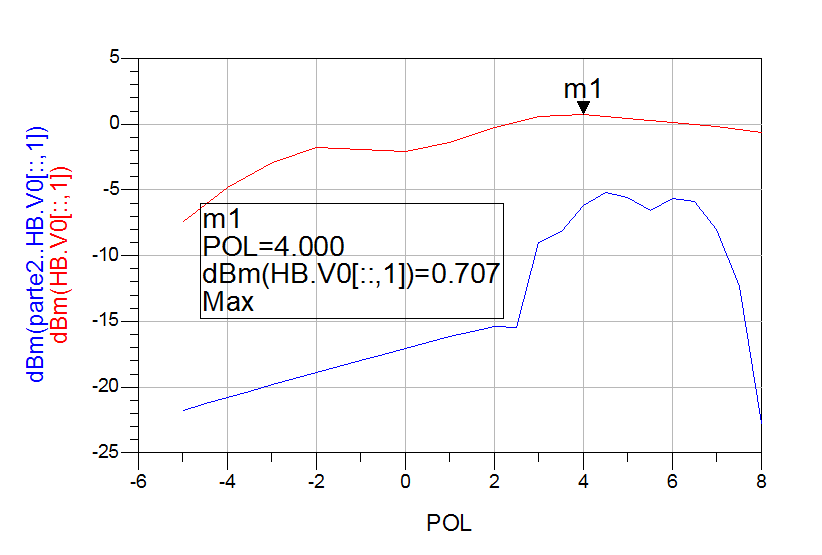
\includegraphics[keepaspectratio=true, scale=0.45]{exps/GT_1}
\vspace{-0.5em}
\caption{Gráfico do ganho de transdução de conversão em função de $ P_{\text{OLDISP}}\left(\omega_{OL}\right) $, com filtro (a vermelho) e sem filtro (a azul).}
\vspace{-0.8em}
\label{fig:GT_1}
\end{figure}

Como se pode ver, o valor de $ P_{\text{OLDISP}}\left(\omega_{OL}\right) $ que maximiza o ganho de transdução de conversão passou de 4.5 dBm para 4 dBm. \todo{why?}

É também possível comparar os espectros de potência, Figura \ref{fig:EP_1}.

\begin{figure}[h]
\centering
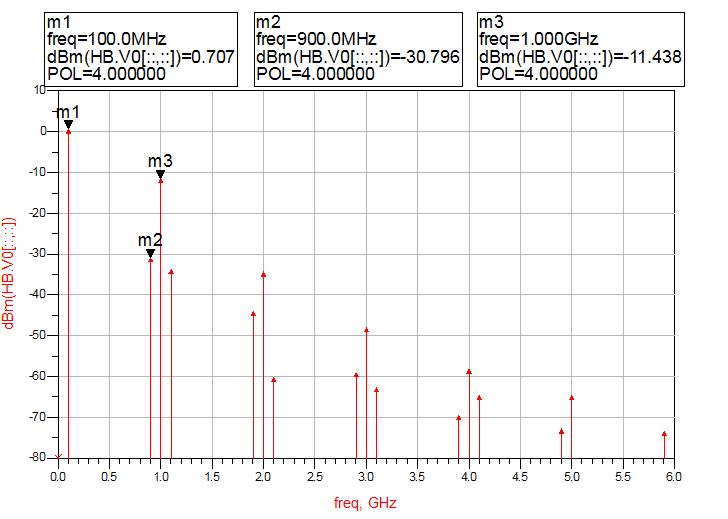
\includegraphics[keepaspectratio=true, scale=0.45]{exps/EP_1}
\vspace{-0.5em}
\caption{Espectros de potência após a inserção do filtro.}
\vspace{-0.8em}
\label{fig:EP_1}
\end{figure}

A partir da Figura \ref{fig:EP_1} pode-se calcular os valores dos isolamentos $OL-RF$ e $OL-FI$ com a introdução do filtro.

\begin{table}[h]
	\centering
	\caption{Valor dos isolamentos.}
	\vspace{-1.5mm}
	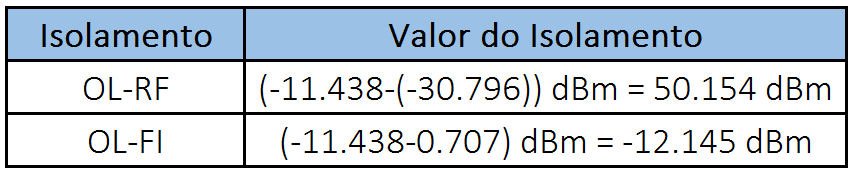
\includegraphics[keepaspectratio=true, scale=0.40]{teoricas/isolamentosFiltro}
\end{table}

\todo{explicar diferenças nos isolamentos}

À semelhança do que foi feito anteriormente calcula-se também o valor do ganho de conversão \todo{mesmo problema de antes - como fazer?}

\subsection{Componentes da tensão $V_{BE}$ e da corrente $I_{C}$} 

Pretende-se agora obter as componentes da tensão $v_{BE}$ e da corrente $I_{C}$ nas frequências $f_{OL}$, $f_{RF}$ e $f_{FI}$.

\begin{figure}[h]
\centering
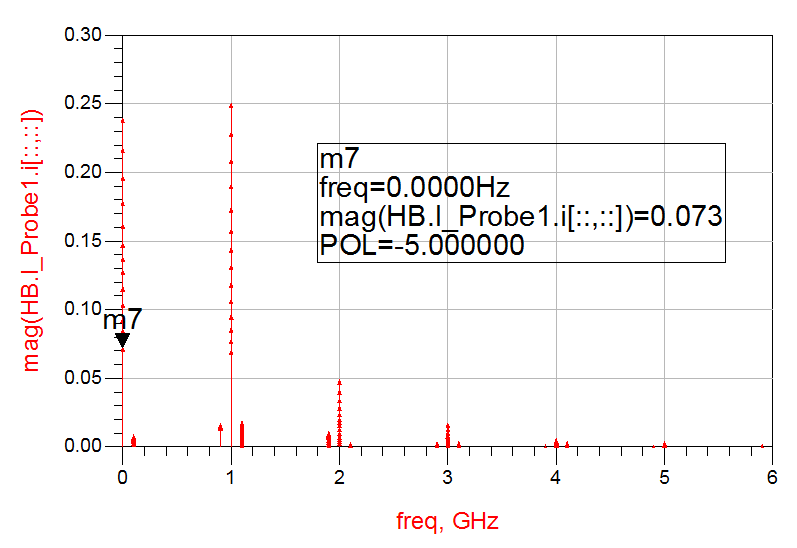
\includegraphics[keepaspectratio=true, scale=0.45]{exps/ID}
\vspace{-0.5em}
\caption{Espectros de potência da corrente $I_{C}$ em função de $ P_{\text{OLDISP}\left(\omega_{OL}\right)} $.}
\vspace{-0.8em}
\label{fig:ID}
\end{figure}

\begin{figure}[h]
\centering
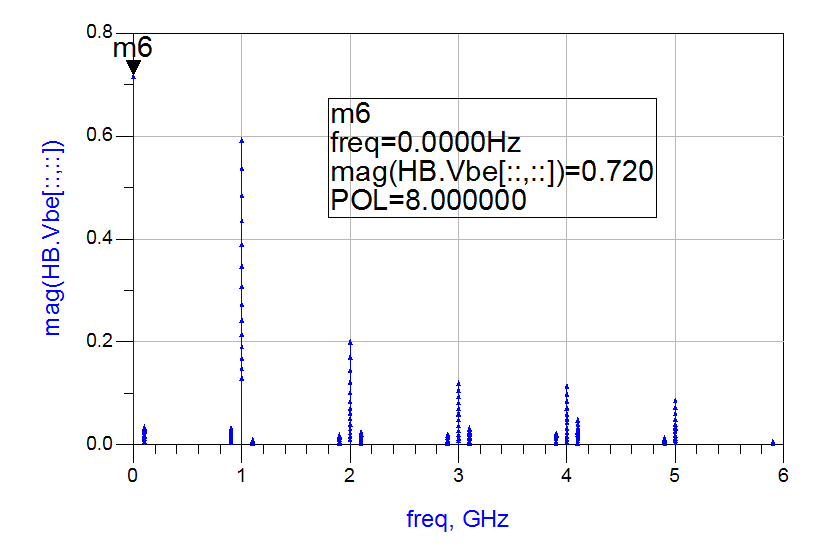
\includegraphics[keepaspectratio=true, scale=0.45]{exps/Vbe}
\vspace{-0.5em}
\caption{Espectros de potência da corrente $V_{BE}$ em função de $ P_{\text{OLDISP}\left(\omega_{OL}\right)} $.}
\vspace{-0.8em}
\label{fig:Vbe}
\end{figure}

A corrente $I_{C}$ para a qual o circuito foi dimensionado é de 55 mA, no entanto verifica-se que o valor obtido para a frequência de trabalho é de \todo{valor experimental}. De facto, isto ocorre porque a corrente $I_{C}$ é uma função de $ P_{\text{OLDISP}}\left(\omega_{OL}\right) $, ou seja, o circuito é na verdade dimensionado para uma corrente $I_{CQ}$ (a componente contínua) mas depois no misturador passa para $I_{C}$. Este fenómeno é inevitável mas trabalha a nosso favor porque faz aumentar o ganho.

Relativamente ao valor de $V_{BE}$ este já não é uma função de $ P_{\text{OLDISP}}\left(\omega_{OL}\right) $ porque o circuito foi polarizado em tensão, ou seja, o seu valor foi forçado. Assim se explica que para uma frequência de 1 GHz o valor obtido corresponda ao dimensionado.

\todo{margarida mete as explicações do caderno}

Pode-se também obter o valor do ganho de compressão a -1 dB do ganho de transdução de conversão, ou seja, registar a 

\begin{figure}[h]
\centering
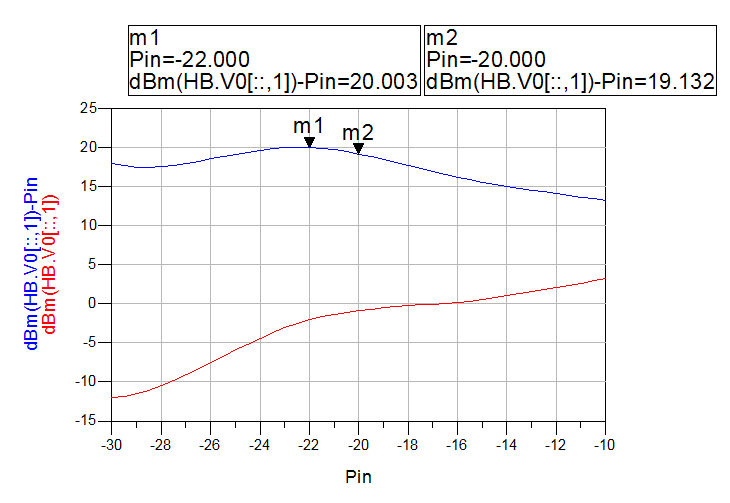
\includegraphics[keepaspectratio=true, scale=0.45]{exps/Compression}
\vspace{-0.5em}
\caption{Ponto de Compressão a $-1dB$ do ganho de conversão.}
\vspace{-0.8em}
\label{fig:Compressao}
\end{figure}


\todo{explicar}

\subsection{Acoplador de Wilkinson}

\paragraph{Malha de Entrada Adaptada} \hspace{0pt} 

Usando as equações da Figura \ref{fig:Eq}, é possível, na simulação do circuito, observar as impedâncias de de entrada de RF e de OL, Figura \ref{fig:Imp_OL_RF}.

\begin{figure}[h]
\centering
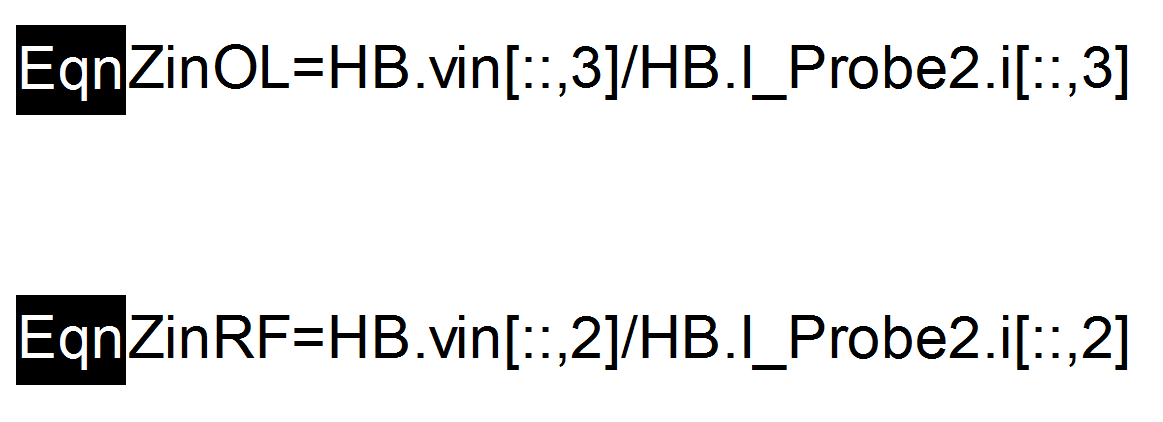
\includegraphics[keepaspectratio=true, scale=0.2]{exps/Eq}
\vspace{-0.5em}
\caption{Equações das impedâncias de entrada de OL (em cima) e RF (em baixo).}
\vspace{-0.8em}
\label{fig:Eq}
\end{figure}


\begin{figure}[h]
\centering
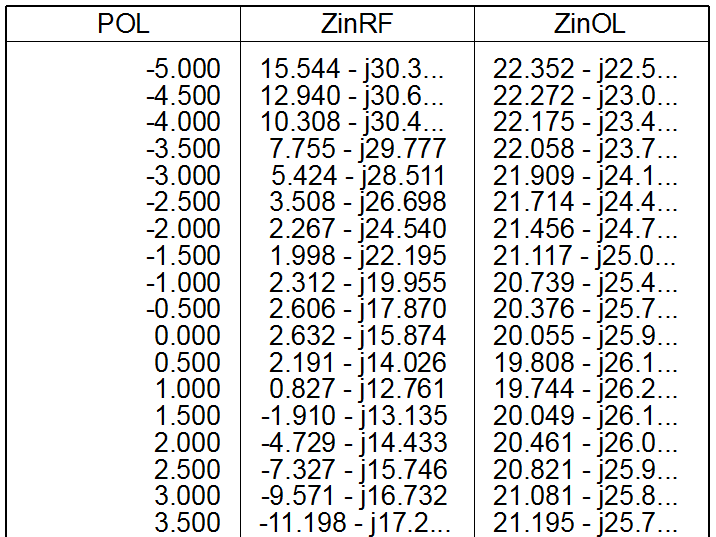
\includegraphics[keepaspectratio=true, scale=0.45]{exps/Z_20}
\vspace{-0.5em}
\caption{Valores das impedâncias de entrada de OL (à direita) e RF (à esquerda).}
\vspace{-0.8em}
\label{fig:Imp_OL_RF}
\end{figure}

Ao observar a Figura \ref{fig:Imp_OL_RF}, é possível verificar que não se verificam oscilações no valor de $ Z_{\text{in}_{OL}} $ com a variação de $ P_{\text{OLDISP}}\left(\omega_{OL}\right) $, \todo{qual o impacto teórico que isto tem}. Verificando a Figura \ref{fig:GT_1}, o valor de $ P_{\text{OLDISP}}\left(\omega_{OL}\right) $ que corresponde ao máximo do ganho de transdução é 4. No entanto, nesta situação, ficar-se-ia com uma componente real negativa de $ Z_{\text{in}_{RF}} $, sendo então necessário encontrar outro máximo do ganho de transdução, que corresponda a uma componente real positiva para $ Zin_{RF} $.

\begin{figure}[h]
\centering
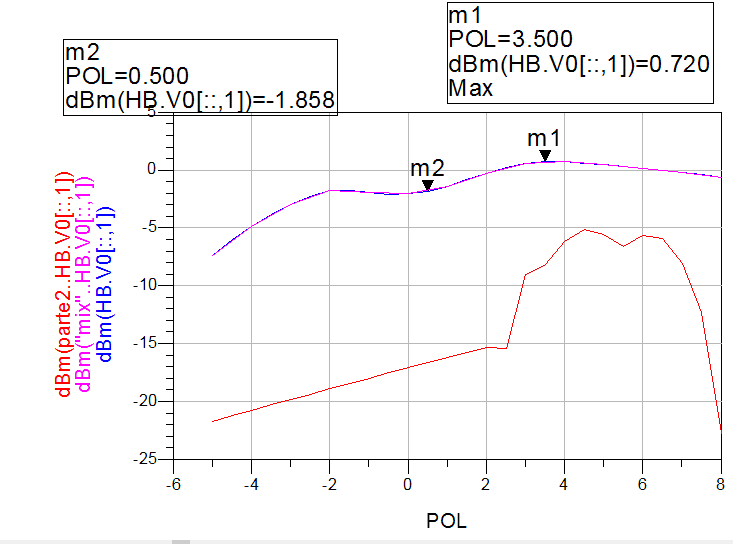
\includegraphics[keepaspectratio=true, scale=0.45]{exps/GT_20}
\vspace{-0.5em}
\caption{Gráfico do ganho de transdução de conversão em função de $ P_{OLDISP(\omega_{OL})} $, encontrar o novo máximo.}
\vspace{-0.8em}
\label{fig:GT_20}
\end{figure}

O novo valor encontrado para $ P_{\text{OLDISP}}\left(\omega_{OL}\right) $ na Figura \ref{fig:GT_20} é de TAL e, como se pode verificar na Figura \ref{fig:Imp_OL_RF}, representa um valor de $ Z_{\text{in}_{RF}} $ cuja componente real é positiva, $ 2.191 -j14.026 \Omega $.

Usando a ferramenta SmithChart do ADS é possível então determinar que adaptação se deve realizar na malha de entrada. Em primeiro lugar é necessário normalizar o valor da impedância de entrada de RF, ou seja, dividir o seu valor pela impedância característica (50 $\Omega$), de onde se obtém o valor $0.04382 -j0.28052$, como se pode observar na Figura \ref{fig:M_adapt}.

\begin{figure}[h]
\centering
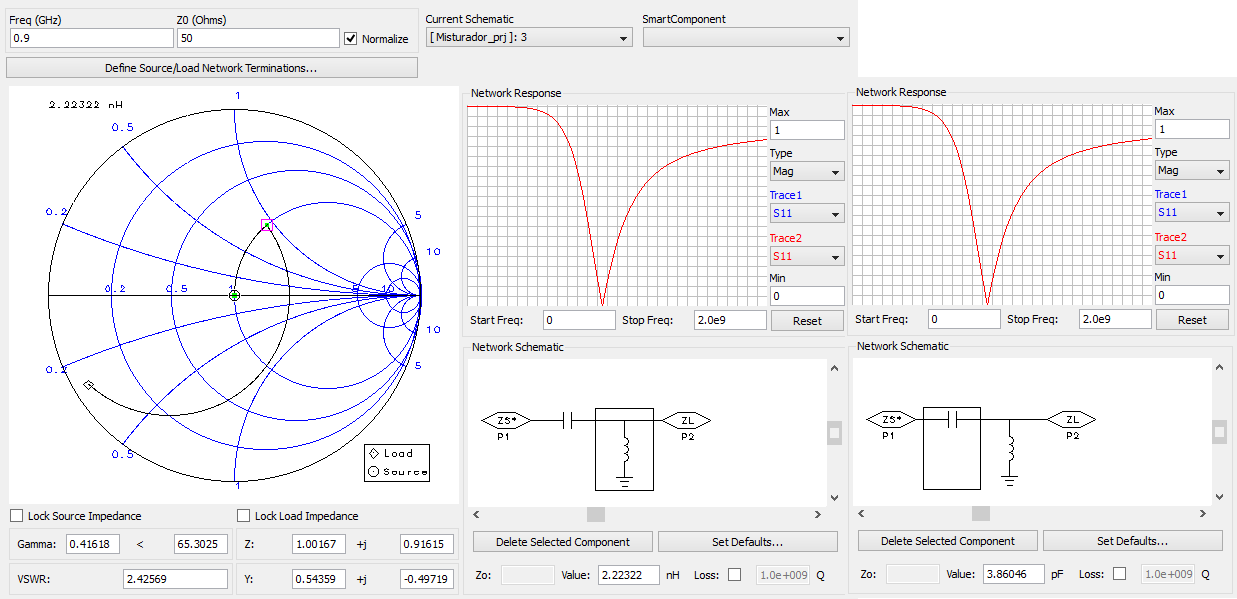
\includegraphics[keepaspectratio=true, scale=0.45]{exps/M_adapt}
\vspace{-0.5em}
\caption{Cálculo da malha de adaptação.}
\vspace{-0.8em}
\label{fig:M_adapt}
\end{figure}

Assim, foram alcançado novos valores para os componentes $L_{CH1}$ e $C_{1}$, que são apresentados na Tabela \todo{referir a tabela que vais fazer}.

\begin{table}[h]
	\centering
	\caption{Valores utilizados para os condensadores de desacoplamento e bobines de bloqueio.}
	\vspace{-1.5mm}
	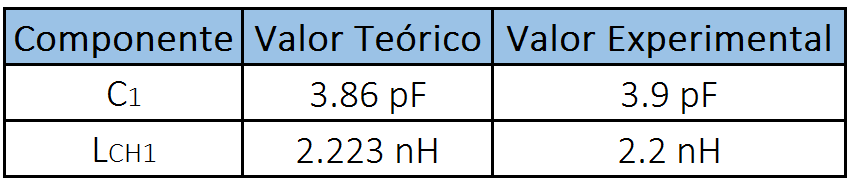
\includegraphics[keepaspectratio=true, scale=0.40]{teoricas/componentes2}
\end{table}

\todo{Faz uma tabela igual à tabela \ref{tab:cap_ind} bobine ch1 e condensador1, são os que estao na imagem 2.223nH e 3.86pF, como valores usados mete 2.2nH e 3.9pF}

Com esta alteração o gráfico de transdução sofreu alterações, que podem se observadas na Figura \ref{fig:GT_21}.

\begin{figure}[h]
\centering
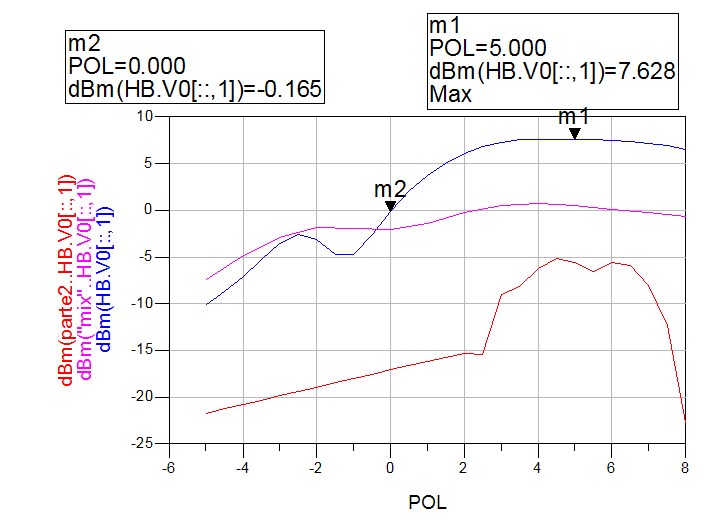
\includegraphics[keepaspectratio=true, scale=0.45]{exps/GT_21}
\vspace{-0.5em}
\caption{Gráfico do ganho de transdução em função de $ P_{\text{OLDISP}}\left(\omega_{OL}\right) $ sem filtro (a vermelho), com filtro e sem malha de adaptação (a roxo)e s/ malha de adaptação, azul- c/malha de adaptação e filtro)}
\vspace{-0.8em}
\label{fig:GT_21}
\end{figure}

É possível então verificar que quando $ P_{\text{OLDISP}}\left(\omega_{OL}\right) $ é de '0', obtém-se um ganho de transdução desejável(0dB). Podemos também verificar que  os valores das impedâncias de entrada de RF e OL(Figura \ref{}) mantêm-se estáveis sem se verificar grandes oscilações.

\begin{figure}[h]
\centering
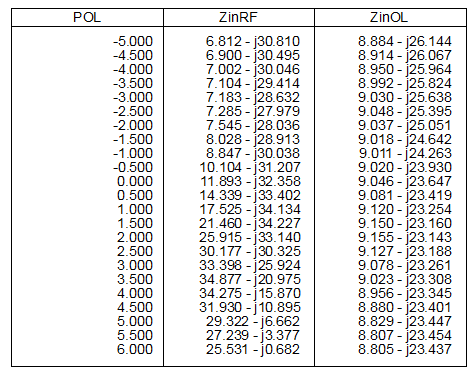
\includegraphics[keepaspectratio=true, scale=0.45]{exps/Z_21}
\vspace{-0.5em}
\caption{Valores das Impedâncias de entrada de OL(Direita) e RF(Esquerda) após da adaptação da malha de entrada.}
\vspace{-0.8em}
\label{fig:Imp_OL_RF_21}
\end{figure}


\paragraph{Acoplamento de Wilkinson} \hspace{0pt} 

Após a adaptação na malha de entrada, substituiu-se o elemento \texttt{Pwr Split} por um aop\textit{Wilkinson}(Figura ), que foi dimensionado para a frequência $ f_{RF} $.

\begin{figure}[h]
\centering
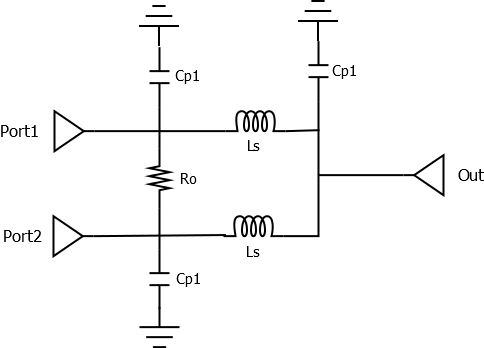
\includegraphics[keepaspectratio=true, scale=0.45]{teoricas/Wilkinson}
\vspace{-0.5em}
\caption{Acoplador de Wilkinson correspondente a um bloco \texttt{Pwr Split}.}
\vspace{-0.8em}
\label{fig:Wilk}
\end{figure}


De modo a obter um power spliter que trabalhe na frequência de $900MHz$($ f_{RF} $), os componentes apresentados na Figura \ref{fig:Wilk} foram dimensionados de acordo com as Equações \ref{eq:Wilk_L}, \ref{eq:Wilk_C} e \ref{eq:Wilk_R}. 

\begin{equation}
L_{s}=frac{Z_{0}}{2 \pi f_{RF}}
\label{eq:Wilk_L}
\end{equation}

\begin{equation}
C_{p2}=2C_{p1}=frac{2}{2 \pi f_{RF}Z_{0}}
\label{eq:Wilk_C}
\end{equation}

\begin{equation}
R_{0}=2Z_{0}
\label{eq:Wilk_R}
\end{equation}


Os valores obtidos através das Equações \ref{eq:Wilk_L}, \ref{eq:Wilk_C} e \ref{eq:Wilk_R}, e os valores usados no circuito para os componentes do acoplador de Wilkinson estão representados na Tabela.

\todo{Fazer tabela com valores, perguntar ao GUI}

Após de colocar os componentes e obter o circuito total (filtro de FI, malha de entrada adaptada e acoplador de Wilkinson), representado na Figura \ref{fig:Circuito_3}, é possível obter o gráfico da do ganho de transdução (Figura \ref{fig:GT_3}).



\begin{figure}[h]
\centering
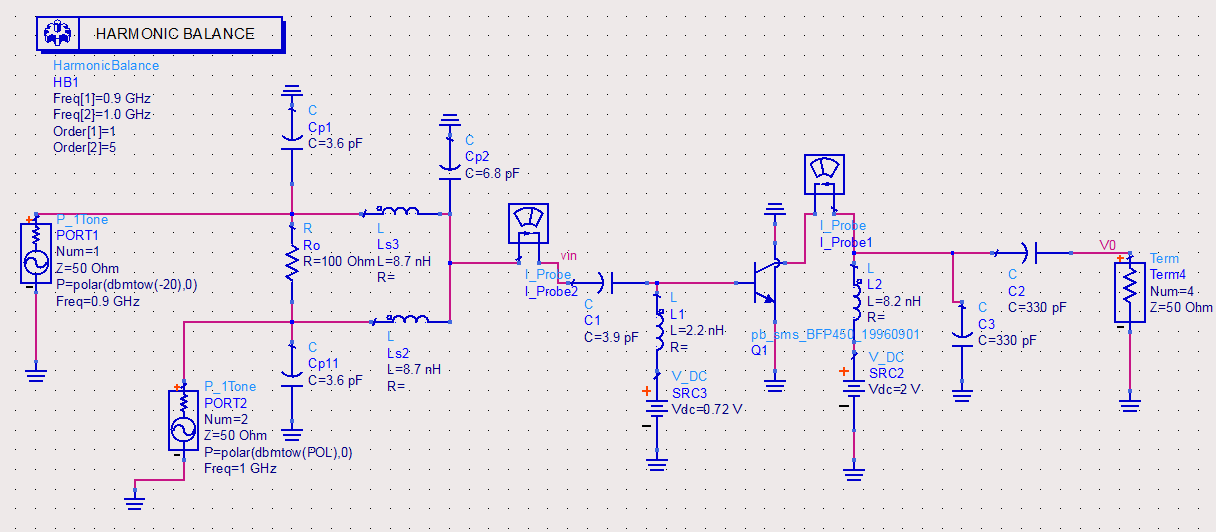
\includegraphics[keepaspectratio=true, scale=0.45]{exps/Circuito_3}
\vspace{-0.5em}
\caption{Circuito final do misturador.}
\vspace{-0.8em}
\label{fig:Circuito_3}
\end{figure}



\begin{figure}[h]
\centering
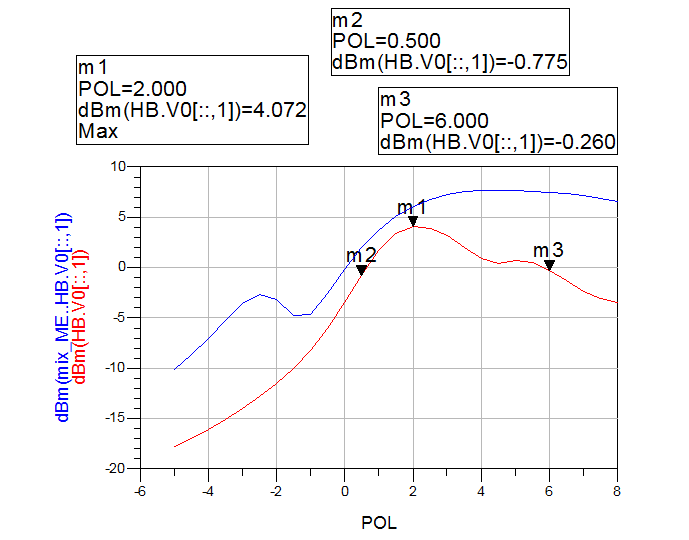
\includegraphics[keepaspectratio=true, scale=0.45]{exps/GT_3}
\vspace{-0.5em}
\caption{Gráfico do ganho de transdução em função de $ P_{\text{OLDISP}\left(\omega_{OL}\right)} $, sem acoplador de Wilkinson (a azul), com acoplador de Wilkinson (a vermelho).}
\vspace{-0.8em}
\label{fig:GT_3}
\end{figure}

Como se pode observar na Figura \ref{fig:GT_3}, é possível perceber que após a introdução do acoplador de Wilkinson no circuito, este perdeu ganho, no entanto contínua a ter valores satisfatórios, tal como um máximo do ganho de transdução de 4.072 dBm para um valor de $ P_{\text{OLDISP}\left(\omega_{OL}\right)} $ de 2 dBm, para valores de $ P_{\text{OLDISP}\left(\omega_{OL}\right)} $ aproximadamente entre 0.5 e 6, temos um ganho de transdução maior que 0 dbM. 

Para um valor de $ P_{\text{OLDISP}\left(\omega_{OL}\right)} $ de 2 (correspondente ao máximo do ganho de transdução) foi obtido o espectro de potências (\ref{fig:EP_3}).

\begin{figure}[h]
\centering
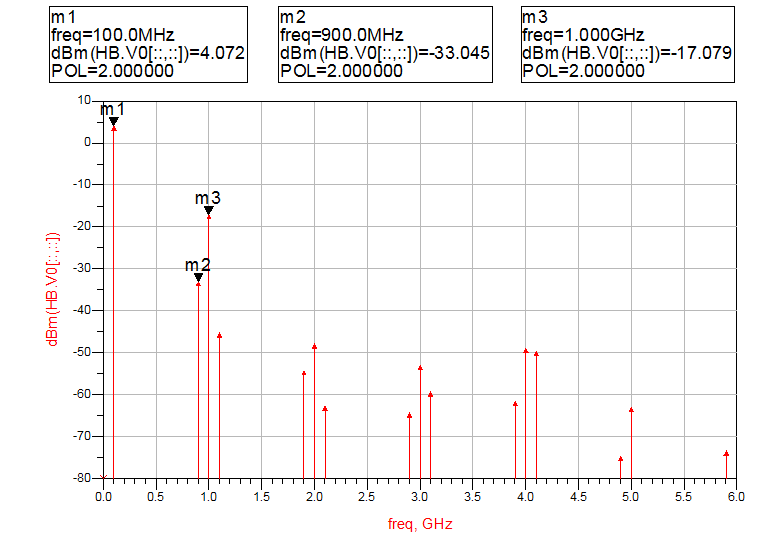
\includegraphics[keepaspectratio=true, scale=0.45]{exps/EP_3}
\vspace{-0.5em}
\caption{Espectros de potência após a inserção do acoplamento de Wilkinson.}
\vspace{-0.8em}
\label{fig:EP_3}
\end{figure}

\todo{Comentar as diferenças depois de sabermos como se calcula os ganhos}

\subsection{Máscara para fabrico}

De modo a obter a máscara para fabrico do circuito é necessário em primeiro lugar obter, através da ferramenta \texttt{Tune}, o comportamento desejado do circuito, e posteriormente substituir os componentes por \texttt{MGAP}.

\paragraph{Linhas e Descontinuidades} \hspace{0pt} 

Em primeiro lugar atribui-se a todas as linhas uma largura de 0.5mm e um comprimento de 1mm, usando depois a ferramenta \texttt{Tune} se necessário.



\paragraph{Condensadores, Bobines e Transistor} \hspace{0pt} 

\section{Conclusões}


\end{document}